\chapter{Lagrange's Theorem and Orbit-Stabilizer Theorem}
\label{ch-lagranges-theorem}


\section{Lagrange's Theorem}

Let $\calh$ be a subgroup of a finite
group $\calg$ (i.e., $\calh\le \calg$)



$g \calh = \{gh| h\in \calh\}=$ {\bf left coset} with coset representative $g$


$\calg/\calh=\{g\calh| g\in \calg\}=\{g\calh| g\in \calg:\calh\}$

$\calg:\calh=$ set of {\bf coset representatives}



The {\bf Lagrange table} is a table with
rows labelled by $g\in \calg:\calh$, columns
labelled by $h\in \calh$, and table entries equal to $gh$.

\begin{claim}Every element of $\calg$ appears exactly once in the Lagrange Table. Therefore\footnote{Eq.(\ref{eq-finite-lagrange}) is for finite groups. For infinite Lie groups,
the order of each group
is replace by the dimension of the Lie algebra vector space: $dim(\ger{g})=dim(\ger{g}/\ger{h}) \; dim (\ger{h})$,
where $\ger{g}=\ger{g}/\ger{h}+\ger{h}$}

\beq
|\calg|=|\calg:\calh| \; |\calh|
\label{eq-finite-lagrange}
\eeq
\end{claim}
\proof

If $x\in \calg$,
then
$x\in x\calh=g\calh$ for some $g\in \calg:\calh$.  So every $x\in \calg$ appears at least in one coset.

Suppose $x$ appears in 2 cosets $g_1\calh$ and $g_2\calh$.
\beq
 g_1h_1=g_2h_2\eeq
so
\beq
g_2^{-1} g_1= h_2 h_1^{-1}\in \calh
\eeq
Hence, 
\beq
g_2^{-1} g_1 \calh = \calh\implies g_2\calh = g_1\calh
\eeq
\qed

A group $\calg$ is {\bf abelian} if $g_1 g_2=g_2 g_1$ for all $g_1,g_2\in  \calg$.

$\calh$ is  a {\bf normal}
subgroup of $\calg$ (i.e., $\calh\trianglelefteq \calg$)
iff $g\calh=\calh g$ (i.e., $g\calh g^{-1}=\calh$)
for all $g\in \calg$.
All subgroups  $\calh$ of an abelian group $\calg$  are
normal subgroups.

$\calg=$ all symmetries.

$\calh=$ symmetries for a given reference state

$\calg:\calh=$ a set of reference states that yield all distinct left cosets,
often called the {\bf index set}

$\calg/\calh=$ set of left cosets, often called a
{\bf quotient space or coset space}. Also called {\bf quotient group or coset group} if $\calh$ is a normal
subgroup



Examples:
\begin{enumerate}
\hrule
\item ($\calh$ not normal subgroup)




$
\calg=S_3 = \{e,\ (12),\ (13),\ (23),\ (123),\ (132)\}
$ The symmetric group on 3 letters,


$\calh = \{e,(12)\}$

Cosets

\beq\left\{
\begin{array}{ll}
e\calh &= \{e,(12)\}
\\
(13)\calh &= \{(13),(123)\}
\\
(23)\calh &= \{(23),(132)\}
\end{array}
\right.
\eeq

$\calg:\calh =
\{e,\ (13),\ (23)\}$ coset representatives. 

\beq
|\calg|= 6, \quad |\calg:\calh|=3, \quad |\calh|=2
\eeq





In this example, $\calh$ is not a normal subgroup of $\calg$
because 
\beq
(13)\calh = \{(13),\underbrace{(13)(12)}
_{(123)}\}
\eeq

and

\beq
\calh(13)
=\{(13),\underbrace{(12)(13)}
_{(213)}\}
\eeq
are not equal.

\hrule
\item ($\calh$ normal because $\calg$ is abelian)


$\calg= Z_6=\{0,1,2,3,4,5\}$
 under addition mod 6.

$\calh=\{0,3\}$

$\calg$ is abelian so every subgroup of $\calg$ is normal

$\calg:\calh=\{0,1,2\}$, coset representatives

Cosets

\beq
\left\{
\begin{array}{ll}
0+ \calh=\{0,3\}
\\
1+ \calh=\{1,4\}
\\
2+ \calh=\{2,5\}
\end{array}
\right.
\eeq

\hrule
\item ($\calh$ is normal subgroup even though $\calg$ is not abelian)

$S_3^e = \{e,(123),(132)\}$, even number of cycles

$S_3^o=\{(12),(13),(23)\}$, odd number of cycles

$\calg=S_3=S_3^o \cup S_3^e$



$
\calh = S_3^e.
$



$S_3^e \trianglelefteq S_3$ because $\s S_3^e =S_3^e \s =S_3^o$
for all $\s \in S_3$

$\calg:\calh=\{e, (12)\}$ coset representatives


Cosets

\beq
\left\{
\begin{array}{ll}
e\calh &= S_3^e
\\
(12)\calh&= S_3^o
\end{array}
\right.
\eeq

\beq
S_3 / S_3^e \cong  Z_2
\eeq

\end{enumerate}

\section{Orbit-Stabilizer Theorem}


Let a group $\calg$ act on a set $X$ by an action $\odot$. This means that $\odot: \calg\times X\rarrow X$ and $(g,x)\mapsto g\odot x$. Usually the {\bf action} $\odot$ is {\bf group conjugation}. $g\odot x= g x g^{-1}$. In the special case  of Lagrange's theorem, $X=\calg$ and $g\odot x=gx$.

$Stab(x)
=\{ g \in \calg | g\odot x = x \}
$= {\bf Stabilizer of $x$}, the symmetries of $x$, group operations that keep $x$ fixed or \qt{stabilized}.

$O(x)=\{g\odot x| g\in \calg \}=$ {\bf Orbit of $x$}, all possible projections of $x$ via $g\in \calg$.

Fig.\ref{fig-orbit-stab} represents  $O(x)$ and $Stab(x)$ pictorially.

\begin{figure}[h!]
\centering
\includegraphics[width=4in]
{lagranges-theorem/orbit-stab.png}
\caption{Pictorial representation of $O(x)$ and $Stab(x)$}
\label{fig-orbit-stab}
\end{figure}

\begin{claim}(Orbit-Stabilizer theorem for single point $x\in X$)
\beq
|\calg| = |O(x)| \;|Stab(x)|
\eeq
\end{claim}
\proof
\qed

$Z(\calg)=\{z\in \calg| gzg^{-1}=z \text{ for all }g\in \calg\}=$ {\bf center of $\calg$}

Suppose $\calh$ is a subgroup of $\calg$ (i.e., $\calh\leq \calg$) and the action is group conjugation.
There are two ways of generalizing $Stab(x)$, to define it
 for a subgroup $\calh$, instead of a
single point $x$

\beq
\left\{
\begin{array}{l}
\cup_{h\in \calh}Stab(h)=
\cup_{h\in \calh}
\{g\in \calg| ghg^{-1}=h\}
=C_\calg(\calh)\quad
\begin{array}{l}\text{\bf centralizer} 
\\  \text{\bf(a.k.a. commutant)}
\end{array}
\\
Stab(\calh)=\{g\in \calg| g\calh g^{-1}=\calh\})=N_\calg(\calh)\quad \text{\bf normalizer}
\end{array}
\right.
\eeq


Both $C_\calg(\calh)$ and $N_\calg(\calh)$ are subgroups of $\calg$.
Furthermore, $C_\calg(\calh)$ is a subgroup of $N_\calg(\calh)$
so

 \beq
Z(\calg)
\leq C_\calg(\calh)\leq N_\calg(\calh)\leq \calg
\eeq

$C_\calg(\calh)$ contains elements of $\calg$ that commute
with every element of $\calh$. That's why commutant
is a good name for it. The  elements of
a normalizer, on the other hand, may not commute with some  elements of $\calh$.

 $N_\calg(\calh)$ is the biggest subset of $\calg$ that leaves the subgroup $\calh$ fixed under conjugation.
 If $\calh$ is a normal subgroup of $\calg$,
then $N_\calg(\calh)=\calg$.



$O(\calh)=\cup_{h\in \calh}O(h)=$ projections (orbits) of
structure(subgroup) $\calh$ instead of single point $\calh$


\begin{claim}(Orbit-Stabilizer theorem for subgroup $\calh\leq \calg$)
\beq
|\calg| = |O(\calh)| \;|\underbrace{Stab(\calh)}_{N_\calg(\calh)}|
\eeq
\end{claim}
\proof
\qed

Suppose $\calg$ is a group and $\calh$ is a  subgroup of $\calg$.

For any two $a,b\in \calg$, define $a\sim b$ if $a=gbg^{-1}$ for some $g\in \calg$. This is an
equivalence relation that partitions  $\calg$
into disjoint classes. Now define 

$CC(x)=\{gxg^{-1}|g\in \calg\}=$ {\bf conjugacy class (CC) of $x\in \calg$}.

$CC(\calh)=\{g\calh g^{-1}|g\in \calg\}=
\bigcup_{h\in \calh}CC(h)=$ {\bf union of CCs of $\calh\leq \calg$}.

The orbit (for conjugacy action) and the conjugacy class
are the same thing. 


\beq
CC(x)= O(x)= \calg:Stab(x)
\eeq

\beq CC(\calh)= O(\calh)=\calg:Stab(\calh)
\eeq

A normal subgroup $\calh$ of $\calg$ satisfies $g\calh g^{-1}=\calh$
for all $g\in \calg$, so it equals a union of CCs.

\beq
\calh=\bigcup_{x\in X}CC(x)=CC(X)
\eeq
where $X\subset \calh$.
So conjugacy classes are the "atoms" from which normal subgroups are built.

A {\bf central conjugacy class}
is a $CC(x)$ such that $CC(x)\subset Z(\calg)$.
Hence, we must have  $CC(x)=\{x\}$. So central CCs are precisely the singleton sets
$\{x\}$ for all  $x\in Z(\calg)$.
\begin{claim} (sum of class orders)
\beq
|\calg|= |Z(\calg)| +\sum_{x\in X}
\underbrace{|\calg: Stab(x)|}_{|O(x)|}  \eeq
where $X$ contains representatives
of   non-central CCs (i.e., CCs with more than one element)
\end{claim}
\proof
\qed




\hrule
Examples:
\begin{enumerate}
\item 
$\calg= S_3$


$x=(12)$

$Stab(x)=\{e, (12)\}$

$O(x)= \{ (12), (13)(12)(13), (23)(12)(23)\} =
\{
(12), (23), (13)
\}$

\beq
|\calg|=6, |O(x)|=3, |Stab(x)|=2\implies
|\calg| = |O(x)| \;|Stab(x)|
\eeq
\hrule 
\item (sum of class orders)


$\calg=S_3$

conjugacy classes:

$CC_0=\{e\}$, \quad (0 cycles)

$CC_1=\{(12),(23),(13)\}$, \quad (1 cycle)


$CC_2=\{(123),(132)\}$, \quad (2 cycles)

\beq
|\calg|=6, |CC_0|=1,|CC_1|=3, |CC_2|=2
\implies |\calg|= |CC_0| + |CC_1| + |CC_2|
\eeq

\beq
Z(\calg)= \{e\}
\eeq

\beq
Stab((12))=\{e, (12)\}
\implies |S_3:Stab((12))|=6/2=3
\eeq

\beq
Stab((123))=\{(12), (23), (13)\}
\implies |S_3:Stab((123))|=6/3=2
\eeq

\end{enumerate}

\hrule
Applications:
\begin{itemize}
\item Quantum Error Correction

Pauli group =$\{1, \s_x, \s_y, \s_z\}\times\{\pm 1, \pm i\}$. Has 16 elements.

Clifford group
=group generated by $H=\frac{1}{\sqrt{2}}\begin{pmatrix}1&1\\1&-1\end{pmatrix}$
and $S=\begin{pmatrix}1&0\\0&i
\end{pmatrix}$. Has 24 elements

$\calg=$ Pauli or Clifford group

$x$= code state

$O(x)$= orbit (i.e., projections) of code state $x$

$Stab(x)=$ subgroup of $\calg$ that preserves (doesn't change, stabilizes, fixes) code state $x$

$\calh=$ code space, subgroup of $\calg$

$Stab(\calh)=$ subgroup of $\calg$
that fixes code space $\calh$


\item Thermodynamics

$\calg$= group

$x$= single microstate


$O(x)$= set of equivalent microstates=single macrostate

$\ln |O(x)|$= entropy

$Stab(x)=$ subgroup of $\calg$ that preserves (doesn't change, stabilizes, fixes) microstate $x$,
residual symmetry group



\item Lie groups

$\calg$= Lie group

$\calh$= stabilizer, principal fibre

$\calg:\calh=$ base space


$\pi(g)=g\calh=$ projection, fibre

$\pi: \calg\rarrow \calg/\calh=\{g\calh: g\in \calg\}$ fibre bundle

Example

$\calg=SU(2)$

$\calh=U(1)$ fibre

$\calg:\calh=S^2$= two sphere, base space




\end{itemize}
